\begin{figure}[!htbp]\centering
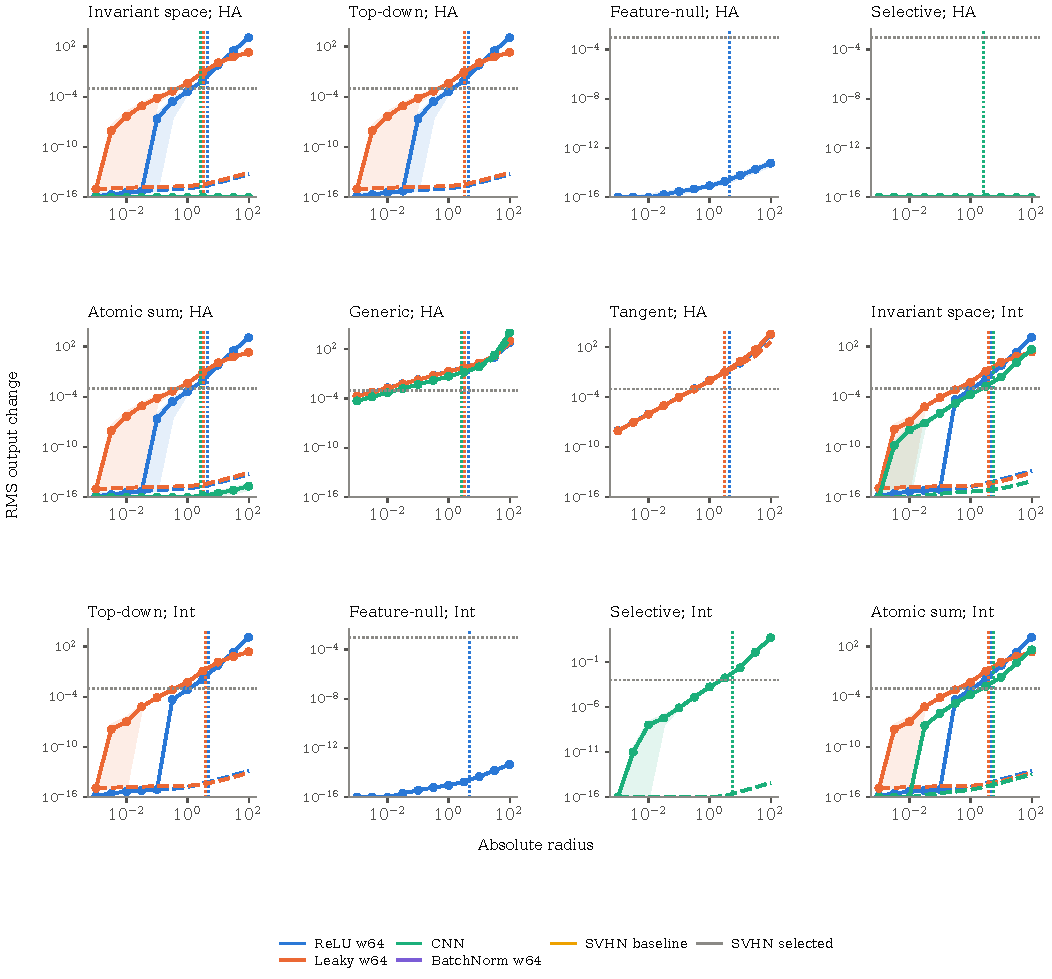
\includegraphics[width=6.313in]{rays_joint_0.pdf}
\caption{Absolute-radius responses across architectures and activations. Each panel fixes the training stage and direction family; only width 64 is shown for leaky ReLU. The Invariant subspace panels combine MLP bottom-up constructions with the CNN received-space construction; Selective panels retain the separate CNN selective candidates. Solid and dashed curves give actual and frozen responses, averaged over seed medians, with seed ranges shaded. Dotted vertical lines mark one tenth of the network norm; the horizontal dotted line marks output change $10^{-3}$. Missing curves indicate unmeasured model--stage combinations.}\label{fig:appendix-ray-comparison}
\end{figure}
\begin{figure}[!htbp]\centering
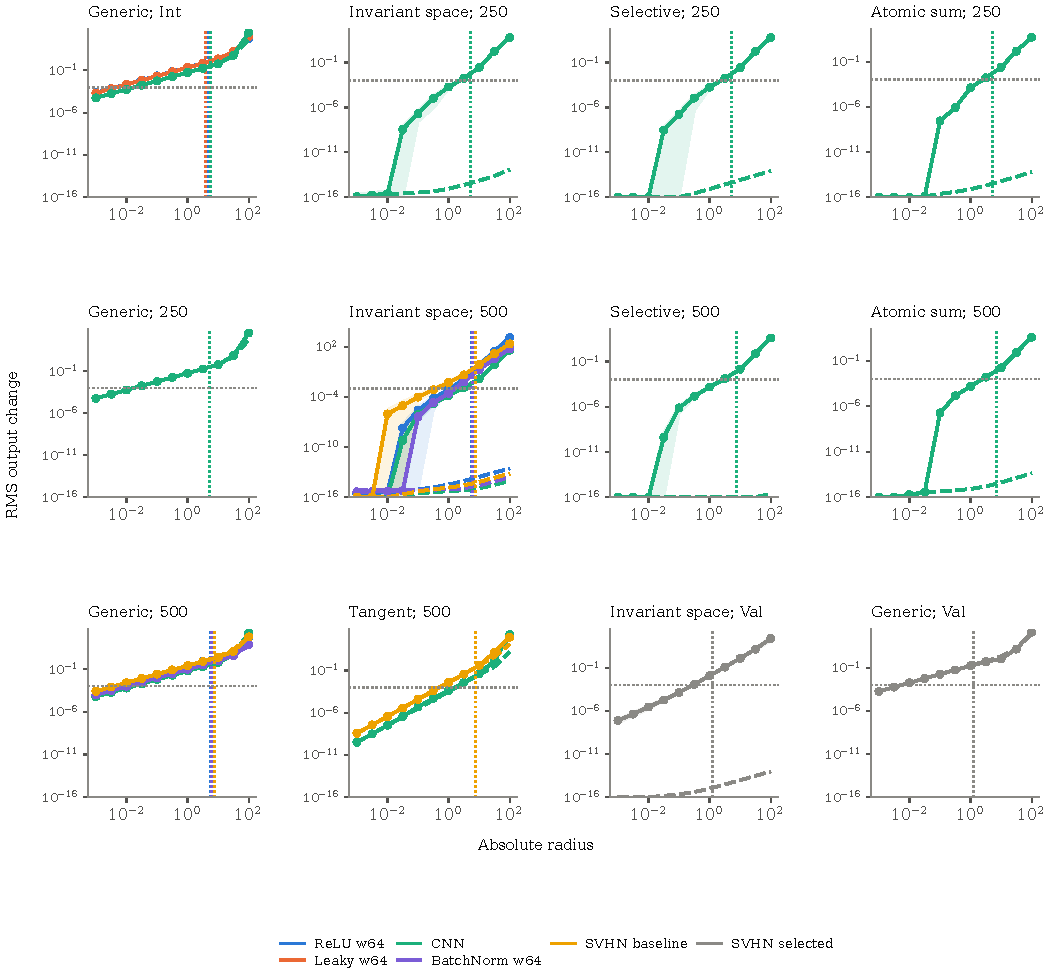
\includegraphics[width=6.313in]{rays_joint_1.pdf}
\caption{Additional stages and direction families, with the conventions of Figure~\ref{fig:appendix-ray-comparison}.}
\end{figure}
\FloatBarrier
